\section{Analysis}
% CONTENT GOAL: Analyze retrieval coverage, final product fix evidence, efficiency, and retained failure modes.
% QUESTIONS FOR AUTHORS: Which causal interpretations are supported by the fix diff and preflight? Which remain hypotheses?
% VERIFIED FACT: Retrieval-preflight Top-10 slot coverage changed from 20/38 to 37/38 across the documented general fix.
% VERIFIED FACT: Targeted Candidate Pool, Final-20, and Answer Top-10 each covered 28/30 slots under a different statistical denominator.
% EVIDENCE: docs/omni-context-paper-evidence-v1/architecture/final-product-fix.md
% EVIDENCE: docs/omni-context-paper-evidence-v1/metrics/targeted-7-summary.json

\begin{figure*}[t]
  \centering
  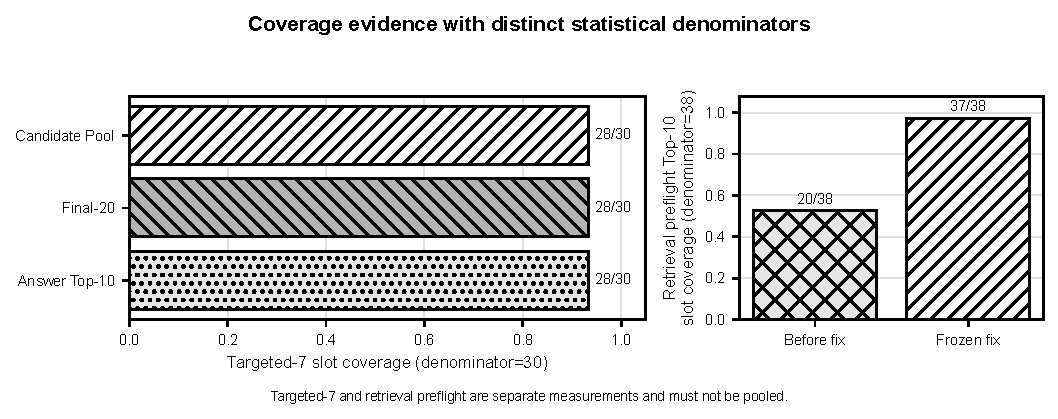
\includegraphics[width=\textwidth]{../figures/coverage-funnel.pdf}
  \caption{Coverage evidence with Targeted and retrieval-preflight denominators kept separate.}
  \label{fig:coverage}
\end{figure*}

\begin{figure*}[t]
  \centering
  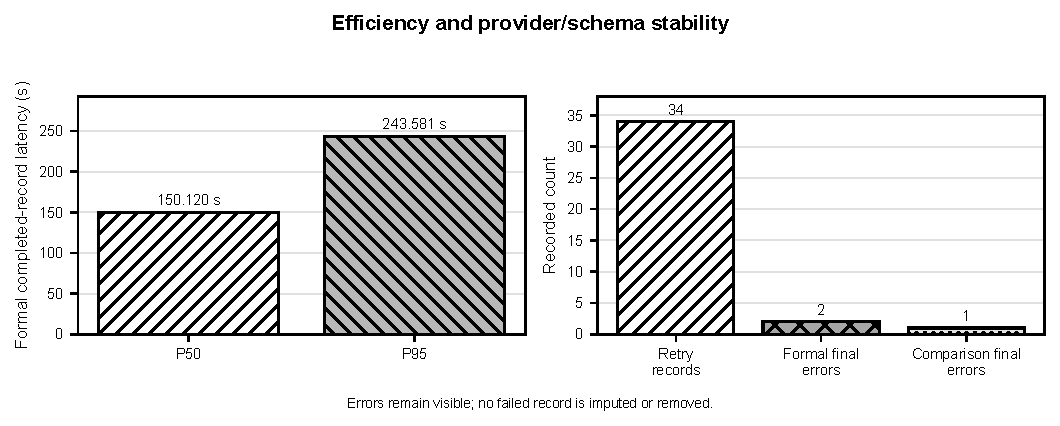
\includegraphics[width=\textwidth]{../figures/latency-summary.pdf}
  \caption{Formal latency and retained retry/error counts.}
  \label{fig:efficiency}
\end{figure*}

\begin{table}[t]
\centering
\caption{Efficiency and stability facts retained without error smoothing.}
\label{tab:efficiency}
\begin{tabular}{lr}
\toprule Metric & Value \\
\midrule
Formal latency P50 & 150120 ms \\
Formal latency P95 & 243581 ms \\
Retry records & 34 \\
Formal final errors & 2 \\
Comparison final errors & 1 \\
\bottomrule
\end{tabular}
\end{table}

\begin{table*}[t]
\centering\scriptsize
\caption{Terminal errors retained after three prescribed attempts. No failed record entered score aggregation.}
\label{tab:errors}
\begin{tabular}{p{0.20\textwidth}lllclclp{0.18\textwidth}p{0.20\textwidth}}
\toprule Scenario & Eval. & Mode & Error & Attempts & Finish & Scored & Attribution & Paper reporting \\
\midrule
\texttt{\detokenize{formal-v2-memory_evolution-039}} & Formal-250 & Full Omni & JSON truncation & 3 & length/length/length & No & Provider structured-output truncation & Retained terminal error; no score imputed \\
\texttt{\detokenize{formal-v2-memory_evolution-040}} & Formal-250 & Full Omni & JSON truncation & 3 & length/length/length & No & Provider structured-output truncation & Retained terminal error; no score imputed \\
\texttt{\detokenize{formal-v2-conflict_resolution-014}} & Comparison-70 & Retrieval-only & empty source\_ids & 3 & stop/stop/stop & No & Baseline schema robustness & Retained terminal error; no score imputed \\
\bottomrule
\end{tabular}
\end{table*}

\TODO{Author analysis required.}
